\documentclass{article}

\usepackage[letterpaper]{geometry}
\usepackage{siunitx}
\usepackage{amsmath}
\usepackage{amssymb}
\usepackage{graphicx}

\title{4261 HW 1}
\author{Duncan Wilkie}
\date{3 February 2022}

\begin{document}

\maketitle

\section*{1a}
The partition function given corresponds to
\[Z(\beta)=\frac{1}{(2\pi h)^3}\int \exp\left( -\beta\frac{\vec{p}^2}{2m} \right)d\vec{p}\int \exp\left( -\beta k\frac{\vec{x}^2}{2} \right)d\vec{x}\]
The integral in one dimension
\[I=\int_{-\infty}^\infty e^{-ax^2}dx\]
may be calculated by first squaring the integral:
\[I^2=\int_{-\infty}^\infty e^{-ax^2}dx\int_{-\infty}^\infty e^{-ay^2}dy=\int_{-\infty}^\infty\int_{-\infty}^\infty e^{-a(x^2+y^2)}dxdy\]
Transforming to polar coordinates, the Jacobian determinant of which you'll recall is $rdrd\theta$, the above becomes
\[I^2=\int_{0}^{2\pi}\int_0^\infty re^{-ar^2}drd\theta\]
This can be solved trivially by a $u$-substitution $u=r^2$, $du=2rdr$:
\[I^2=2\pi\left( \frac{1}{2}\int_0^\infty e^{-au}du\right)=\pi\left( -\frac{e^{-au}}{a}\bigg|_0^\infty \right)=\frac{\pi}{a}\]
Therefore, the integral is equal to $\sqrt{\frac{\pi}{a}}$.

The integral terms of the partition function are then a product of three such integrals with $a=\frac{\beta}{2m}$ for the three scalar variables of momentum and a product of three such integrals with $a=\frac{\beta k}{2}$ for the three scalar variables of position, i.e.
\[Z(\beta)=\frac{1}{(2\pi h)^3}\left( \sqrt{\frac{\pi}{\beta/2m}} \right)^3\left( \sqrt{\frac{\pi}{\beta k/2}} \right)^3=\frac{m^{3/2}}{h^3\beta^3k^{3/2}}\]

\section*{1b}
The expectation of the energy based on the partition function is
\[\langle E \rangle=-\frac{1}{Z}\frac{\partial Z}{\partial \beta}=\frac{h^3\beta^3k^{3/2}}{m^{3/2}}\frac{3m^{3/2}}{h^3\beta^4k^{3/2}}=\frac{3}{\beta}=3k_BT\]
Differentiating to find the heat capacity,
\[C=\frac{\partial \langle E \rangle}{\partial T}=3k_B\]
as desired.

\section*{2a}
The energies of the eigenstates of a one-dimensional harmonic oscillator are $E_{n1D}=\hbar\omega(n+\frac{1}{2})$, so the energies of the eigenstates in the three-dimensional case are
\[E_n=E_x+E_y+E_z=\hbar\omega\left(n_x+n_y+n_z+\frac{3}{2}\right)\]
implying the partition function is
\[Z(\beta)=\sum_{n_{x},n_{y},n_{z}\geq 0}e^{-\beta\hbar\omega\left( n_x+n_y+n_z+3/2 \right)}=e^{-3\beta\hbar\omega/2}\sum_{n_{x}}e^{-\beta\hbar\omega n_{x}}\sum_{n_{y}}e^{-\beta\hbar\omega n_{y}}\sum_{n_{z}}e^{-\beta\hbar\omega n_{z}}\]
\[=e^{-3\beta\hbar\omega/2}\left( \frac{1}{1-e^{-\beta\hbar\omega}} \right)^{3}\]
The Bose occupation factor is the negative of the term in the cube;
\[n_{B}(x)=\frac{1}{e^{x}-1}\]
Functions with this behavior appear in descriptions of the collective behavior of any particles for which multiple may occupy the same quantum state (so-called bosons).

\section*{2b}
The general expression for the expectation value of the energy is
\[\langle E \rangle=-\frac{1}{Z}\frac{\partial Z}{\partial\beta}=-e^{3\beta\hbar\omega/2}\left( 1-e^{-\beta\hbar\omega} \right)^{3}\left( e^{-3\beta\hbar\omega/2}\left[ -3\hbar\omega e^{-\beta\hbar\omega}\left( \frac{1}{1-e^{-\beta\hbar\omega}} \right)^{4} \right]-\frac{3}{2}\hbar\omega e^{-3\beta\hbar\omega/2}\left( \frac{1}{1-e^{-\beta\hbar\omega}} \right)^{3} \right)\]

\[=\frac{-3\hbar\omega e^{-\beta\hbar\omega}}{e^{-\beta\hbar\omega}-1}+\frac{3}{2}\hbar\omega=3\hbar\omega\left( \frac{1}{e^{\beta\hbar\omega}-1}+\frac{1}{2} \right)\]
The heat capacity is
\[C=\frac{\partial\langle E \rangle}{\partial T}=3\hbar\omega\left( -\frac{\hbar\omega}{k_{B}T^{2}}e^{\beta\hbar\omega}\frac{1}{(e^{\beta\hbar\omega}-1)^{2}} \right)=3k_{B}\left( \beta\hbar\omega \right)^{2}\frac{e^{\beta\hbar\omega}}{(e^{\beta\hbar\omega}-1)^{2}}\]

\section*{2c}
As $\beta\to 0$, and therefore $e^{\beta\hbar\omega}\to 1+\beta\hbar\omega$, the heat capacity becomes
\[C\to 3k_{B}(\beta\hbar\omega)^{2}\frac{1+\beta\hbar\omega}{(\beta\hbar\omega)^{2}}=3k_{B}+3k_{B}\beta\omega\hbar\to 3k_{B}\]
which confirms the law of Dulong-Petit.

\section*{2d}
The heat capacity function with nonsense values of $h$ and $\omega$ is gnuplotted below.
\[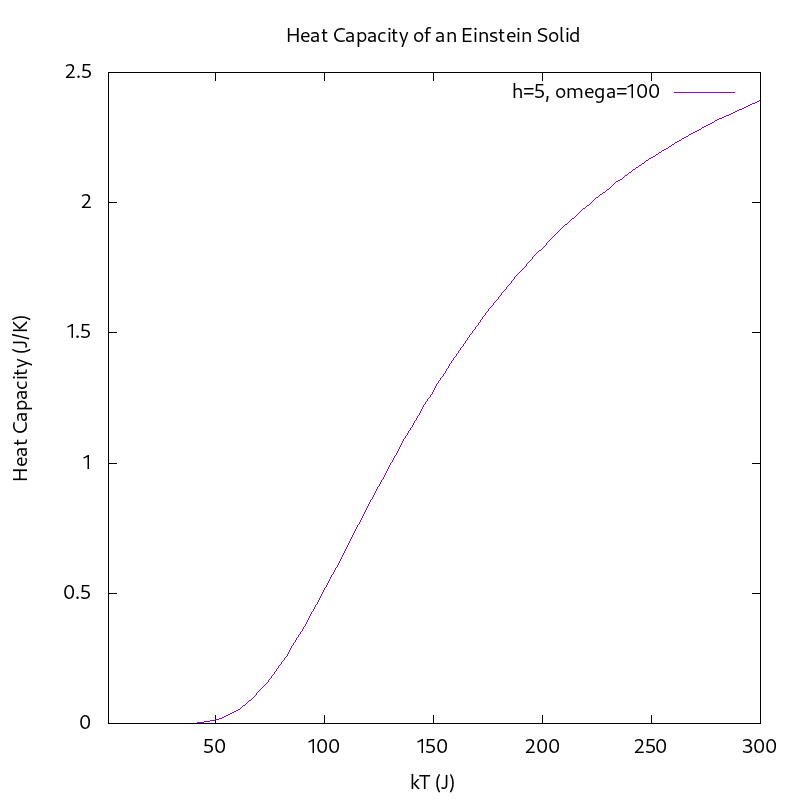
\includegraphics[scale=0.7]{cap.png}\]

\section*{3a}
The Debeye model presumes that heat-capacity-related oscillations behave like sound waves, and are transverse with three polarizations. It then quantizes these waves following Planck, and imposes a maximum frequency cutoff so that the classical $3N$ vibrational degrees of freedom is retained.

\section*{3b}
We presume the oscillation modes of the material have frequencies $\omega(k)=v|k|$, and write down the expectation of the energy of an Einstein solid with this firequency:
\[\langle E \rangle=3\sum_{k}\hbar\omega(k)\left( n_{B}(\beta\hbar\omega(k))+\frac{1}{2} \right)\]
Applying periodic boundary conditions,
\[\langle E \rangle=3\frac{L^{3}}{(2\pi)^{3}}\int\hbar\omega(k)\left( n_{B}(\beta\hbar\omega(k))+\frac{1}{2} \right)dk\]
Transforming to spherical coordinates and plugging in $k=\omega/v$,
\[\langle E \rangle=3\frac{4\pi L^{3}}{(2\pi)^{3}}\int_{0}^{\infty} \left( \frac{\omega^{2}}{v^{2}} \right)\frac{1}{v}\hbar\omega\left( n_{B}(\beta\hbar\omega)+\frac{1}{2} \right)d\omega=\frac{3 L^{3}}{2\pi^{2}}\frac{\hbar}{v^{3}}\int_{0}^{\infty}\frac{\omega^{3}}{e^{\beta\hbar\omega}-1}+\frac{\omega^{3}}{2}d\omega\]
\[\langle E \rangle=\frac{3\hbar L^{3}}{2\pi^{2}v^{3}}\frac{1}{(\beta\hbar)^{4}}\int_{0}^{\infty}\frac{x^{3}}{e^{x}-1}dx +\textrm{$T$-independent constant}\]
Differentiating with respect to $T$,
\[C=\frac{6 L^{3}k_{B}^{4}T^{3}}{\pi^{2}v^{3}\hbar^{3}}\int_{0}^{\infty}\frac{x^{3}}{e^{x}-1}dx\]

\section*{3c}
This is clearly the $T^{3}$ behavior desired for small $T$. However, for high $T$, the cutoff frequency becomes important: no longer do we integrate the expected energy over all $\omega$ but stop at some $\omega_{c}$. The original expression for the energy expectation becomes, using $e^{x}\sim 1+x$ as $x\to 0$,
\[\langle E \rangle=\frac{3\hbar L^{3}}{2\pi^{2}v^{3}}\int_{0}^{\omega_{c}}\omega^{3}\frac{k_{B}T}{\hbar\omega}d\omega+\textrm{$T$-independent constant}\]
The integral is now a finite constant, and so $\langle E \rangle\sim T$ as $T\to\infty$ or $C=\textrm{constant}$, recovering the $C=3Nk_{B}$ behavior of Dulong-Petit.

\section*{3d}
Since the Debeye temperature has the relation
\[C=Nk_{B}\frac{T^{3}}{T_{Debeye}^{3}}\frac{12\pi^{4}}{5}\]
Computing a fit of $c$ against $aT^{3}$ will yield a value for $a$ from which one may compute an estimate of the Debeye temperature. The fit was performed in gnuplot and resulted in \newline$a=(8.0\pm0.2)\times 10^{-4}\hspace{5pt}\si{J/mol\cdot K^{4}}$; a plot of the data and the fit appear below.
\[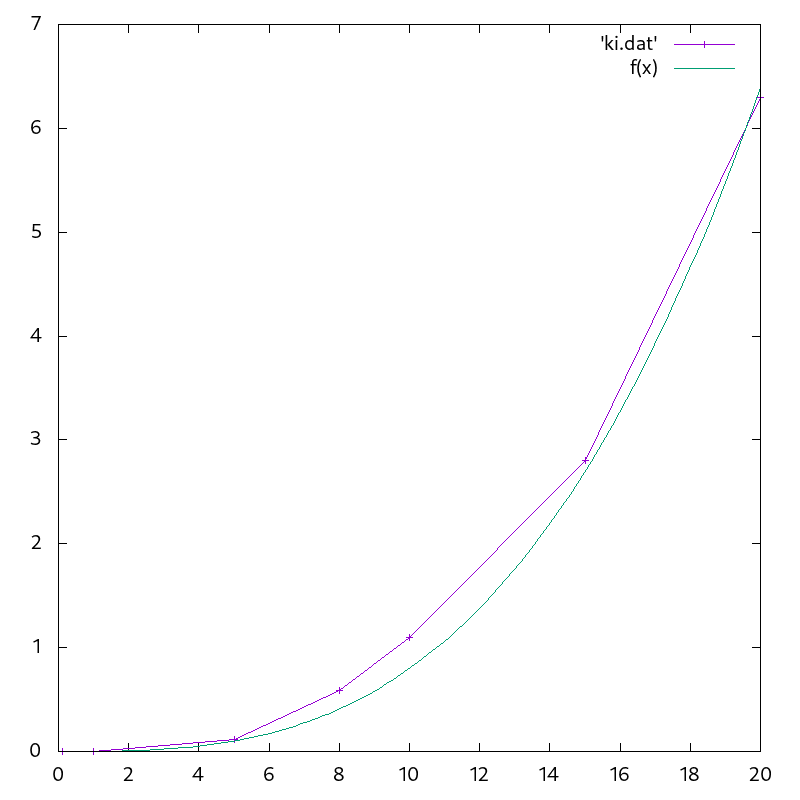
\includegraphics[scale=.7]{fit.png}\]
We expect
\[a=\frac{12\pi^{4}N_{A}k_{B}}{5T_{Debeye}^{3}}\Leftrightarrow T_{Debeye}=\sqrt[3]{\frac{12\pi^{4}N_{A}k_{B}}{5a}}=\sqrt[3]{\frac{12\pi^{4}(\SI{6.28e23}{mol^{-1}})(\SI{1.38e-23}{J/K})}{5(\SI{8.0e-4}{J/mol\cdot K^{4}})}}=136\pm 1\hspace{3pt}\si{K}\]
where the error has been computed by $\sigma_{f(a)}=\frac{\partial f}{\partial a}\sigma_{a}$.
\end{document}
%%% Local Variables:
%%% mode: latex
%%% TeX-master: t
%%% End:
